\title{Article Title}

\author{William Cutler, Jack Donaghue, Haridas Kumarakuru, Don Heiman}

\newcommand{\abstractText}{\noindent
The unique optical properties of the ruby crystal that make it particularly effective as a lasing medium were measured using an inexpensive setup. Ruby’s absorption of visible light was shown to be strongest at \SI{420}{\nm} and \SI{550}{\nm}, corresponding to its physical appearance as translucent and pink. While the ruby crystal was illuminated with a \SI{532}{\nm} green laser, the R-line fluorescence peaked at \SI{693.8\pm1.1}{\nm}. Finally, the fluorescence lifetime of ruby was measured by pulsing the laser with a signal generator and capturing the decaying light waveform on a digital oscilloscope via a high-speed photodiode. An exponential decay time-constant of \SI{3.6\pm0.1}{\ms} was obtained and will be discussed further in this paper. 
}

%%%%%%%%%%%%%%%%%
% Configuration %
%%%%%%%%%%%%%%%%%

\documentclass[12pt, a4paper, twocolumn]{article}
\usepackage{xurl}
\usepackage[comma,sort&compress]{natbib}
\usepackage{abstract}
\usepackage[separate-uncertainty=true]{siunitx}
\usepackage{graphicx}
\renewcommand{\abstractnamefont}{\normalfont\bfseries}
\renewcommand{\abstracttextfont}{\normalfont\small\itshape}
\usepackage{lipsum}

% Any configuration that should be done before the end of the preamble:
\usepackage{hyperref}
\hypersetup{colorlinks=true, urlcolor=blue, linkcolor=blue, citecolor=blue}

\begin{document}

%%%%%%%%%%%%
% Abstract %
%%%%%%%%%%%%

\twocolumn[
  \begin{@twocolumnfalse}
    \maketitle
    \begin{abstract}
      \abstractText
      \newline
      \newline
    \end{abstract}
  \end{@twocolumnfalse}
]

%%%%%%%%%%%
% Article %
%%%%%%%%%%%

\section{Introduction}
The absorption and fluorescence emission spectra have long been used to identify, characterize, and study materials \cite{BrittanicaSpectroscopy}. In lasing mediums such as ruby, these properties govern its excitation and emission spectra respectively. Studies of ruby absorption typically use a spectrophotometer and measure two broad absorption peaks centered near \SI{410}{\nm} and \SI{550}{\nm} \cite{Esposti,Kusuma,Song}. Devices with high resolution (\SI{0.5}{\nm} slit width) additionally detect a small doublet absorption peak near \SI{694}{\nm}. Song et. al. find absorption peaks at \SI{410}{\nm} and \SI{550}{\nm}, and calculates an absorption coefficient from these values according to Beer-Lambert's law.

The room temperature fluorescence spectrum of ruby has been reported well throughout the early 1900's with a double peak at \SI{692.7}{\nm} and \SI{694.2}{\nm}, corresponding to the characteristic $R_1$ and $R_2$ lines \cite{Kumari, Mani}. With lower resolution instruments, only a single primary peak was detected at \SI{694.2}{\nm} by Esposti et. al. Other fluorescence lines have been detected near these peaks at 671, 688, 695, and \SI{710}{\nm} \cite{Kusuma}.

The effectiveness of ruby as a lasing medium depends on its ability to maintain a population inversion between the ground state and the meta-stable state. The stability of this meta-stable state can be measured by the fluorescence lifetime, which relates to how long the crystal will fluoresce in the absence of pumping, and therefore the time for which there is a size-able meta-stable population. Whereas most materials have nano or picosecond fluorescence lifetimes \cite{Berezin}, ruby’s fluorescence lasts milliseconds, and long enough to hold a population inversion for a working laser.

\begin{figure}[t]
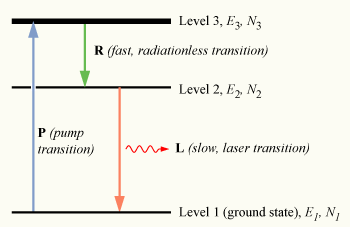
\includegraphics[width=\linewidth]{Population-inversion-3level.png}
\caption{Sample energy level diagram showing three phases of fluorescence: pumping, non-radiative relaxation, and fluorescent relaxation}
\label{fig:populationInversion}
\end{figure}

The fluorescence lifetime of around \SI{3.5}{\ms} is typically reported, but this measurement is dependent on a number of factors. Investigations of the temperature dependence show that lifetime decreases for temperatures above room temperature \cite{Seat, Nelson}. Investigations of the dependence on ruby diameter show an increasing fluorescence lifetime with increased size as emitted photons are reabsorbed more frequently in larger samples \cite{Jones}. The effect of doping concentration changes dramatically with the temperature as found by \cite{Brown}. Brown found that at room temperature, doping concentrations between 0.005\% and 0.1\% yielded lifetimes in the range of 3-\SI{4}{\ms}.


Many investigations use a single-exponential fit to obtain the fluorescence lifetime, but others use a double-exponential fit based on the shape of their residuals \cite{McBane, Jones}. There is also some variation on whether a background constant is accounted for, but without it, we found a lifetime further from the typical \SI{3.5}{\ms} and closer to the \SI{4.2}{\ms} reported by Esposti.

\section{Section2Title}
\lipsum[1]
%%%%%%%%%%%%%%
% References %
%%%%%%%%%%%%%%

\nocite{*}
\bibliographystyle{plain}
\bibliography{reference}

\end{document}

